%%%%%%%%%%%%%%%%%%%%%%%%%%%%%%%%%%%%%%%%%
% Jacobs Landscape Poster
% LaTeX Template
% Version 1.1 (14/06/14)
%
% Created by:
% Computational Physics and Biophysics Group, Jacobs University
% https://teamwork.jacobs-university.de:8443/confluence/display/CoPandBiG/LaTeX+Poster
% 
% Further modified by:
% Nathaniel Johnston (nathaniel@njohnston.ca)
%
% This template has been downloaded from:
% http://www.LaTeXTemplates.com
%
% License:
% CC BY-NC-SA 3.0 (http://creativecommons.org/licenses/by-nc-sa/3.0/)
%
%%%%%%%%%%%%%%%%%%%%%%%%%%%%%%%%%%%%%%%%%

%----------------------------------------------------------------------------------------
%	PACKAGES AND OTHER DOCUMENT CONFIGURATIONS
%----------------------------------------------------------------------------------------

\documentclass[final]{beamer}

\usepackage[scale=1.24]{beamerposter} % Use the beamerposter package for laying out the poster

\usetheme{confposter} % Use the confposter theme supplied with this template

\setbeamercolor{block title}{fg=ngreen,bg=white} % Colors of the block titles
\setbeamercolor{block body}{fg=black,bg=white} % Colors of the body of blocks
\setbeamercolor{block alerted title}{fg=white,bg=dblue!70} % Colors of the highlighted block titles
\setbeamercolor{block alerted body}{fg=black,bg=dblue!10} % Colors of the body of highlighted blocks
% Many more colors are available for use in beamerthemeconfposter.sty

%-----------------------------------------------------------
% Define the column widths and overall poster size
% To set effective sepwid, onecolwid and twocolwid values, first choose how many columns you want and how much separation you want between columns
% In this template, the separation width chosen is 0.024 of the paper width and a 4-column layout
% onecolwid should therefore be (1-(# of columns+1)*sepwid)/# of columns e.g. (1-(4+1)*0.024)/4 = 0.22
% Set twocolwid to be (2*onecolwid)+sepwid = 0.464
% Set threecolwid to be (3*onecolwid)+2*sepwid = 0.708

\newlength{\sepwid}
\newlength{\onecolwid}
\newlength{\twocolwid}
\newlength{\threecolwid}
\setlength{\paperwidth}{48in} % A0 width: 46.8in
\setlength{\paperheight}{36in} % A0 height: 33.1in
\setlength{\sepwid}{0.024\paperwidth} % Separation width (white space) between columns
\setlength{\onecolwid}{0.22\paperwidth} % Width of one column
\setlength{\twocolwid}{0.464\paperwidth} % Width of two columns
\setlength{\threecolwid}{0.708\paperwidth} % Width of three columns
\setlength{\topmargin}{-0.5in} % Reduce the top margin size
%-----------------------------------------------------------

\usepackage{graphicx}  % Required for including images

\usepackage{booktabs} % Top and bottom rules for tables

%----------------------------------------------------------------------------------------
%	TITLE SECTION 
%----------------------------------------------------------------------------------------

\title{ETERNITY: NUMBERS - Silver Ratio $(\delta_s)$} % Poster title

\author{Md Hasibul Huq} % Author(s)

\institute{Department of Computer Science and Software Engineering (CSSE) , Concordia University} % Institution(s)

%----------------------------------------------------------------------------------------

\begin{document}

\addtobeamertemplate{block end}{}{\vspace*{2ex}} % White space under blocks
\addtobeamertemplate{block alerted end}{}{\vspace*{2ex}} % White space under highlighted (alert) blocks

\setlength{\belowcaptionskip}{2ex} % White space under figures
\setlength\belowdisplayshortskip{2ex} % White space under equations

\begin{frame}[t] % The whole poster is enclosed in one beamer frame

\begin{columns}[t] % The whole poster consists of three major columns, the second of which is split into two columns twice - the [t] option aligns each column's content to the top

\begin{column}{\sepwid}\end{column} % Empty spacer column

\begin{column}{\onecolwid} % The first column

%----------------------------------------------------------------------------------------
%	OBJECTIVES
%----------------------------------------------------------------------------------------

\begin{alertblock}{Objectives}

The objective of this project is develop a document of software requirement specification to learn how the industry runs it's operation. Tried to develop a SRS  based on specific criteria. Those are:- 
\begin{itemize}
\item Learn about an irrational number.
\item Interviewing someone related to the specific assigned number
\item Based on the interview analyze the interview. 
\item Develop a Class diagram, a use case diagram, and an activity diagram based on the analysis.
\item Find out user stories from the above mention sources and out of the mention list .
\item Based on the user stories tractability matrix creation
\item Developing a calculator based on the user stories. 
\end{itemize}
The main objective of this project is to integrate the necessary  operation that is not available in calculator but need to support this numbers in calculator.
\end{alertblock}

%----------------------------------------------------------------------------------------
%	INTRODUCTION
%----------------------------------------------------------------------------------------

\begin{block}{Introduction}

This poster provides an understanding of only an irrational  number called Silver Ratio $(\delta_s)$. An irrational  number is  not  a rational  number, it is not possible to express an irrational number as a quotient of two integers \cite{project_des}.

\end{block}

%------------------------------------------------

\begin{figure}
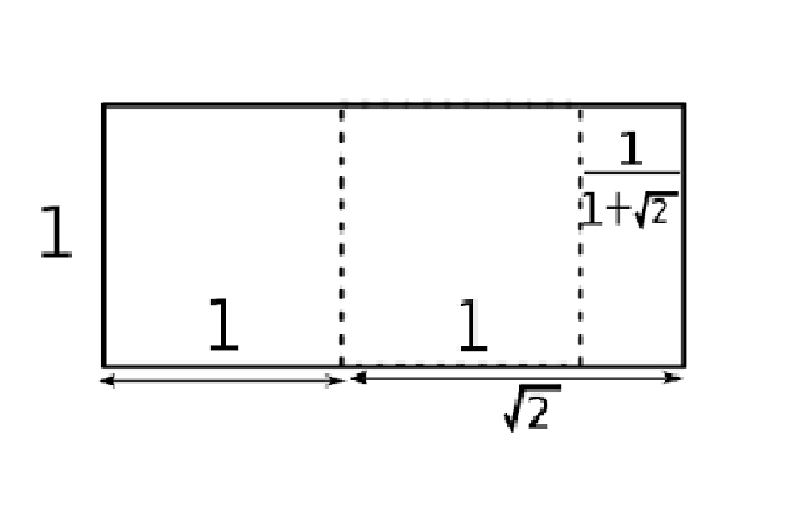
\includegraphics[width=0.8\linewidth]{silver_ratio.png}
\caption{Silver Rectangle}
\end{figure}

%----------------------------------------------------------------------------------------

\end{column} % End of the first column

\begin{column}{\sepwid}\end{column} % Empty spacer column

\begin{column}{\twocolwid} % Begin a column which is two columns wide (column 2)

\begin{columns}[t,totalwidth=\twocolwid] % Split up the two columns wide column

\begin{column}{\onecolwid}\vspace{-.6in} % The first column within column 2 (column 2.1)

%----------------------------------------------------------------------------------------
%	History
%----------------------------------------------------------------------------------------

\begin{block}{History}
Silver Ratio is studied from the time of Greek knowledge, which discusses the fundamental characteristics of the number system. Though it is not used by normal people intentionally. Silver ratio is the limiting of consecutive  of infinite sequence of integers, The silver ratio is presented in a Greek symbol ($\delta_s$).

\end{block}


%----------------------------------------------------------------------------------------

%----------------------------------------------------------------------------------------
%	MATHEMATICAL SECTION
%----------------------------------------------------------------------------------------
\begin{block}{Mathematical Definition}
The value of silver ration is 2.4142135623 \cite{jdc_silver}. A ratio of the sequential sum of smaller number and twice of the larger number, which will produce an infinite sequence and the ration between smaller and larger number will be always same \cite{numberphile_silver}. This can be presented in mathematical equation:- 

\[ \dfrac{2a + b}{a}  = \dfrac{b}{a} = \delta_s \]

It will be easier to understand if it can be compared with Fibonacci number.
In Fibonacci, the smaller and larger number are added to get the next one. 
Example:-

$$1,1,2,3,5,8,13,..$$

For silver ratio, the smaller and twice of the larger number are added to get the next one. Example:-

\[1,2,5,12,29,70,..\] 

Then the latest number is divided  by the previous larger number. 
\end{block}

%----------------------------------------------------------------------------------------
%	Persona
%----------------------------------------------------------------------------------------

\begin{block}{Persona}

\begin{figure}
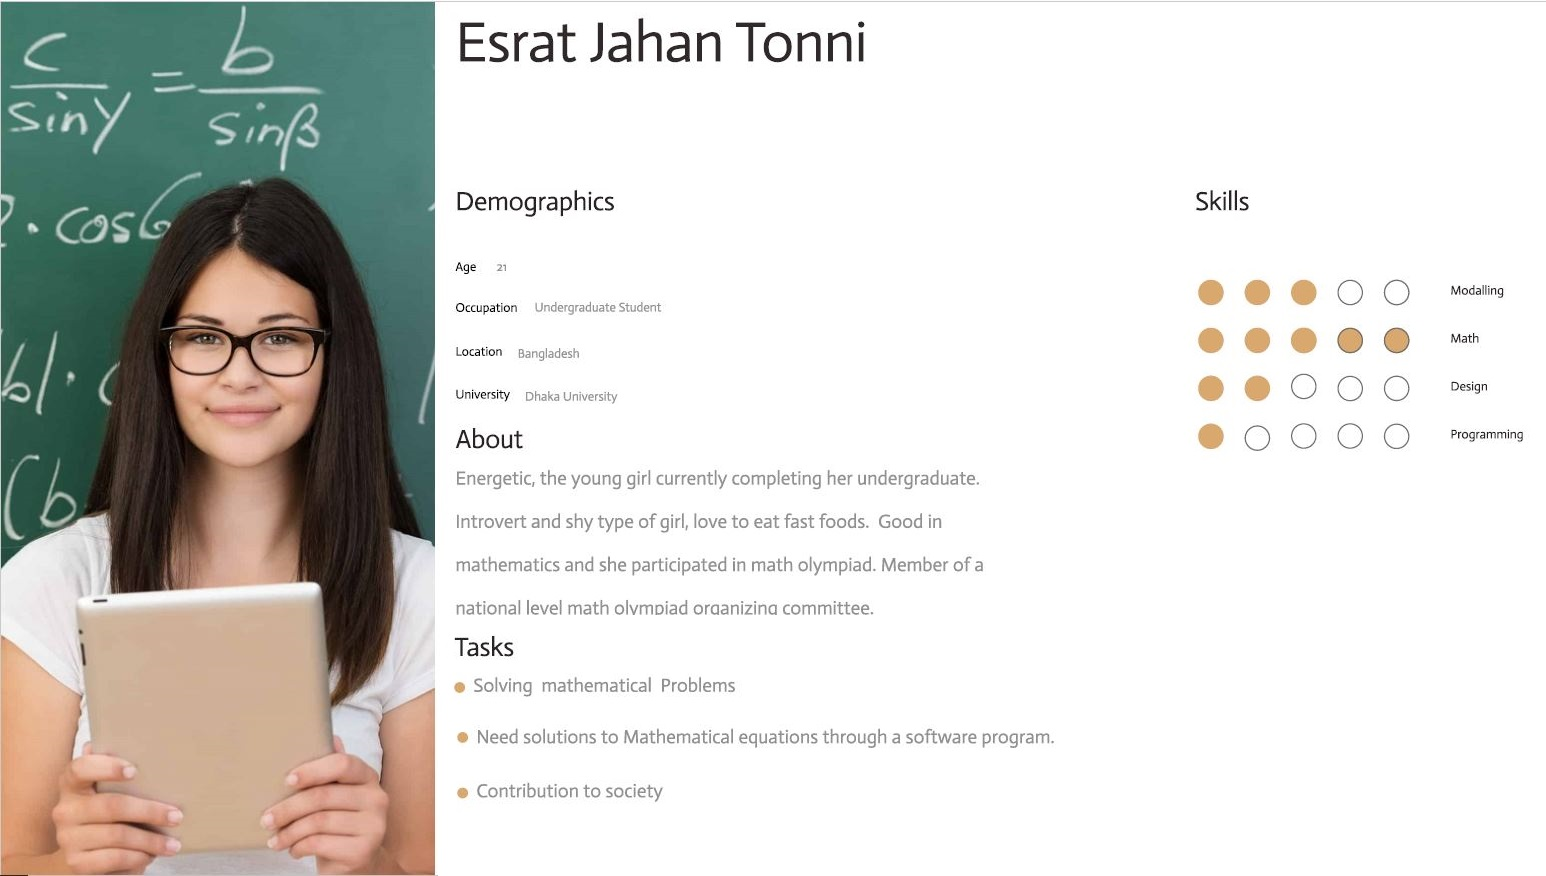
\includegraphics[width=0.8\linewidth]{persona.png}
\caption{Persona of Interviewee}
\end{figure}

\end{block}


%----------------------------------------------------------------------------------------

\end{column} % End of column 2.1

\begin{column}{\onecolwid}\vspace{-.6in} % The second column within column 2 (column 2.2)

%----------------------------------------------------------------------------------------
%	METHODS
%----------------------------------------------------------------------------------------

\begin{block}{Interview  Analysis}
Though the interviewee is not expert in the area of the irrational numbers, She has decent idea about the silver ratio. As she has a math background, she gave a lots of insights about the silver ratio. She is 4th Year student and completed 3 years in math domain. As a math student she has to use calculator almost everyday and she uses scientific calculator for the complex equations. From the interview, it is clear that the silver ratio is used in calculation of geometrical shapes. Also the architect, designer, engineers and Sometimes doctors (Plastic Surgery) uses this. Also stated that in regular scientific calculator the irrational numbers are not available. Then she describe about the silver ratio . which has the value of 4142135623.Its convergent are square triangular numbers, Pell numbers and octagons. According to her it will be good if the irrational numbers are included in the scientific calculator. According to him the calculation can be done here in the scientific calculators but they needs extra effort. But inclusion of these can make few peoples life easier. 


\end{block}

\begin{block}{Documents and Designs}
Instead of all requirements I am providing the number related requirements here. 
\begin{itemize}
\item As an user, I want the button of
silver ratio as number.  So that i
can use it as a number for arithmetic operation.
\item As an  user,  I want  to know the
number for which silver ratio will
be a given number.
\end{itemize}
\begin{figure}
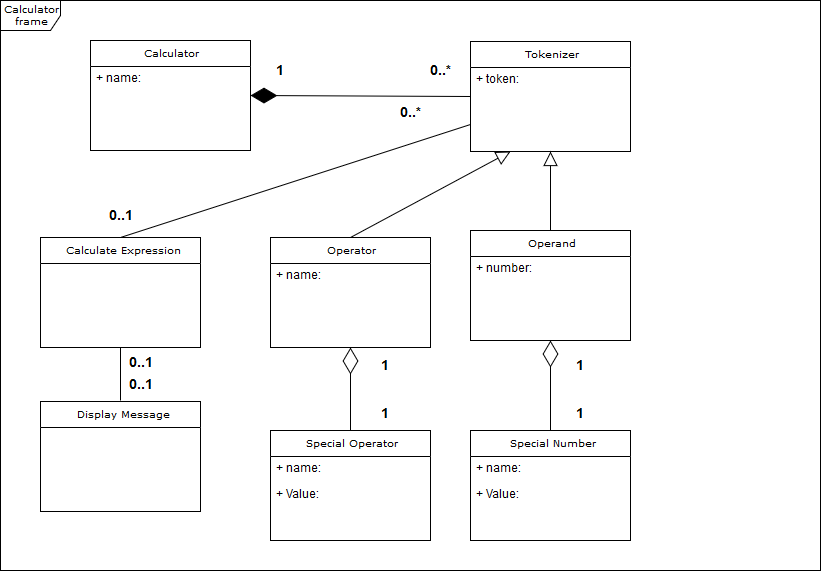
\includegraphics[width=0.8\linewidth]{uml.png}
\caption{Class Diagram}
\end{figure}



\end{block}
%----------------------------------------------------------------------------------------

\end{column} % End of column 2.2

\end{columns} % End of the split of column 2 - any content after this will now take up 2 columns width

%----------------------------------------------------------------------------------------
%	IMPORTANT RESULT
%----------------------------------------------------------------------------------------



%----------------------------------------------------------------------------------------

\end{column} % End of the second column

\begin{column}{\sepwid}\end{column} % Empty spacer column

\begin{column}{\onecolwid} % The third column

\begin{figure}
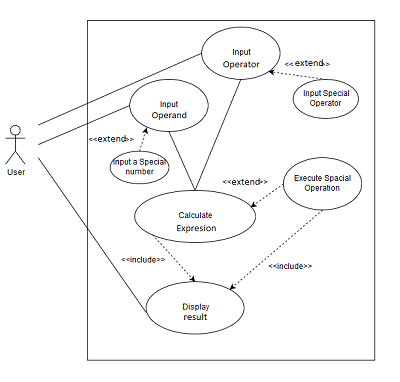
\includegraphics[width=0.25\linewidth]{usecase.png}
\caption{Class Diagram}
\end{figure}
%----------------------------------------------------------------------------------------
%	CONCLUSION
%----------------------------------------------------------------------------------------

\begin{block}{Conclusion}

In this document, the user requirements for the calculator system have been presented to capture basic requirement of a calculator system along with silver ratio.

\end{block}

%----------------------------------------------------------------------------------------
%	REFERENCES
%----------------------------------------------------------------------------------------

\begin{block}{References}

\nocite{*} % Insert publications even if they are not cited in the poster
\small{\bibliographystyle{unsrt}
\bibliography{sample}\vspace{0.75in}}

\end{block}

%----------------------------------------------------------------------------------------
%	ACKNOWLEDGEMENTS
%----------------------------------------------------------------------------------------

\setbeamercolor{block title}{fg=red,bg=white} % Change the block title color

\begin{block}{Acknowledgements}

\small{\rmfamily{I like to show my gratitude to the Pankaj Kamtahn to provide the opportunity to learn new things from the project. I also want to thank my group mates for their valuable contribution to the persona.}} \\

\end{block}

%----------------------------------------------------------------------------------------
%	CONTACT INFORMATION
%----------------------------------------------------------------------------------------

\setbeamercolor{block alerted title}{fg=black,bg=norange} % Change the alert block title colors
\setbeamercolor{block alerted body}{fg=black,bg=white} % Change the alert block body colors

\begin{alertblock}{Contact Information}

\begin{itemize}
\item Web: \href{http://www.hasibulhuq.com}{http://www.hasibulhuq.com}
\item Email: \href{mailto:rafi3170@gmail.com}{rafi3170@gmail.com}
\item Phone: +1 (438) 866 7234
\end{itemize}

\end{alertblock}


%----------------------------------------------------------------------------------------

\end{column} % End of the third column

\end{columns} % End of all the columns in the poster

\end{frame} % End of the enclosing frame

\end{document}
